\documentclass[hyperref={pdfpagemode=FullScreen}]{beamer}
\usepackage[utf8]{inputenc}
\usepackage{multicol}
\usepackage{graphicx}
\usepackage{ragged2e}
\title{Azerbaijan}
\usetheme{Madrid}
\usecolortheme{beaver}
\title{AZERBAIJAN}
\author{Rashad Mahmudov}
\date{3 May 2020}

\begin{document}

\begin{frame}
\titlepage
\end{frame}

\setlength{\columnsep}{0.7cm}
\begin{frame}{Location}
\begin{multicols}{2}
\justifying Republic of Azerbaijan, is a country in the South Caucasus region of Eurasia at the crossroads of Eastern Europe and Western Asia. 

It is bounded by the Caspian Sea to the east, Russia to the north, Georgia to the northwest, Armenia to the west and Iran to the south. 

The exclave of Nakhchivan has an 11 km long border with Turkey in the northwest.

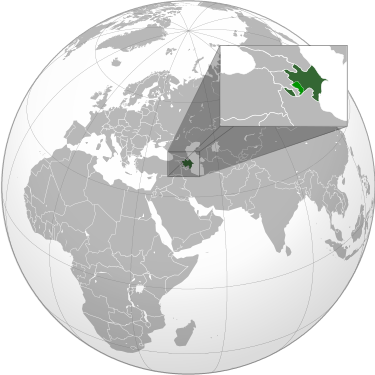
\includegraphics[scale=.42]{img/aze01.png}
\end{multicols}
\end{frame}


\begin{frame}{History}
\begin{alertblock}{Antiquity}
\justifying The earliest evidence of human settlement in  Azerbaijan dates back to the late Stone Age and is related to the Guruchay culture of Azokh Cave. 

The Upper Paleolithic and late Bronze Age cultures are attested in the caves of Tağılar, Damcılı, Zar, Yataq-yeri and in the necropolises of Leylatepe and Saraytepe.
\end{alertblock}
\end{frame}


\begin{frame}{History}
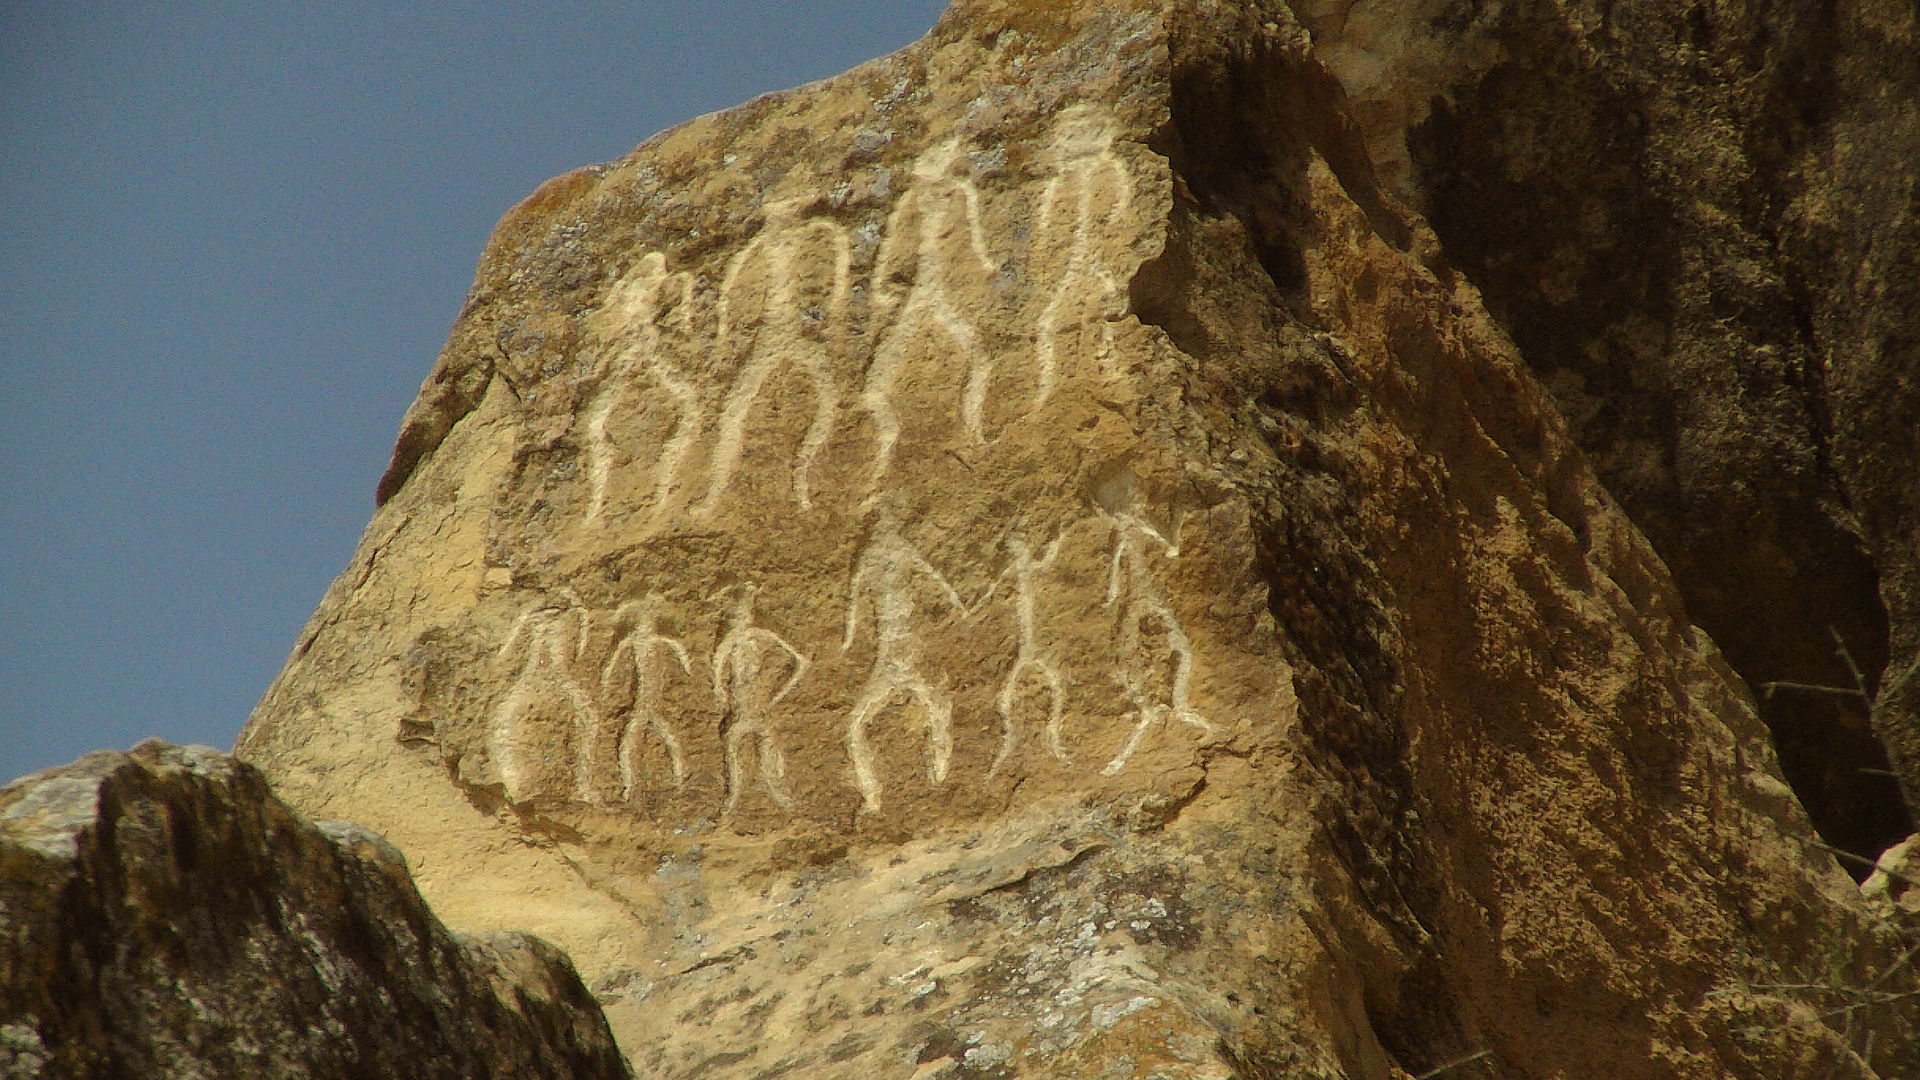
\includegraphics[width=12cm, height=8cm]{img/aze02.jpg}
\end{frame}

\begin{frame}{Cities}
\begin{alertblock}{Baku}
\justifying Baku, the capital city of Azerbaijan, enjoys a number of titles. It is the biggest city in Azerbaijan as well as the largest city in the Caucasus region and on the Caspian Sea. Baku population - 2,262,600
\end{alertblock}
\end{frame}

\begin{frame}{Baku}
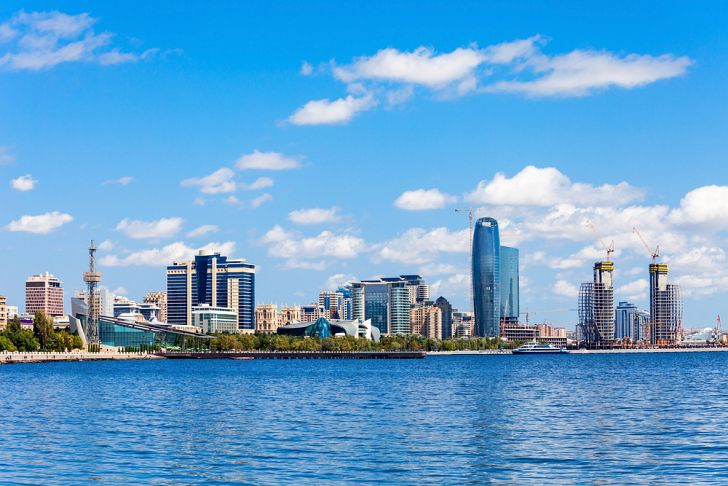
\includegraphics[width=12cm, height=8cm]{img/baku01.jpg}
\end{frame}

\begin{frame}{Baku}
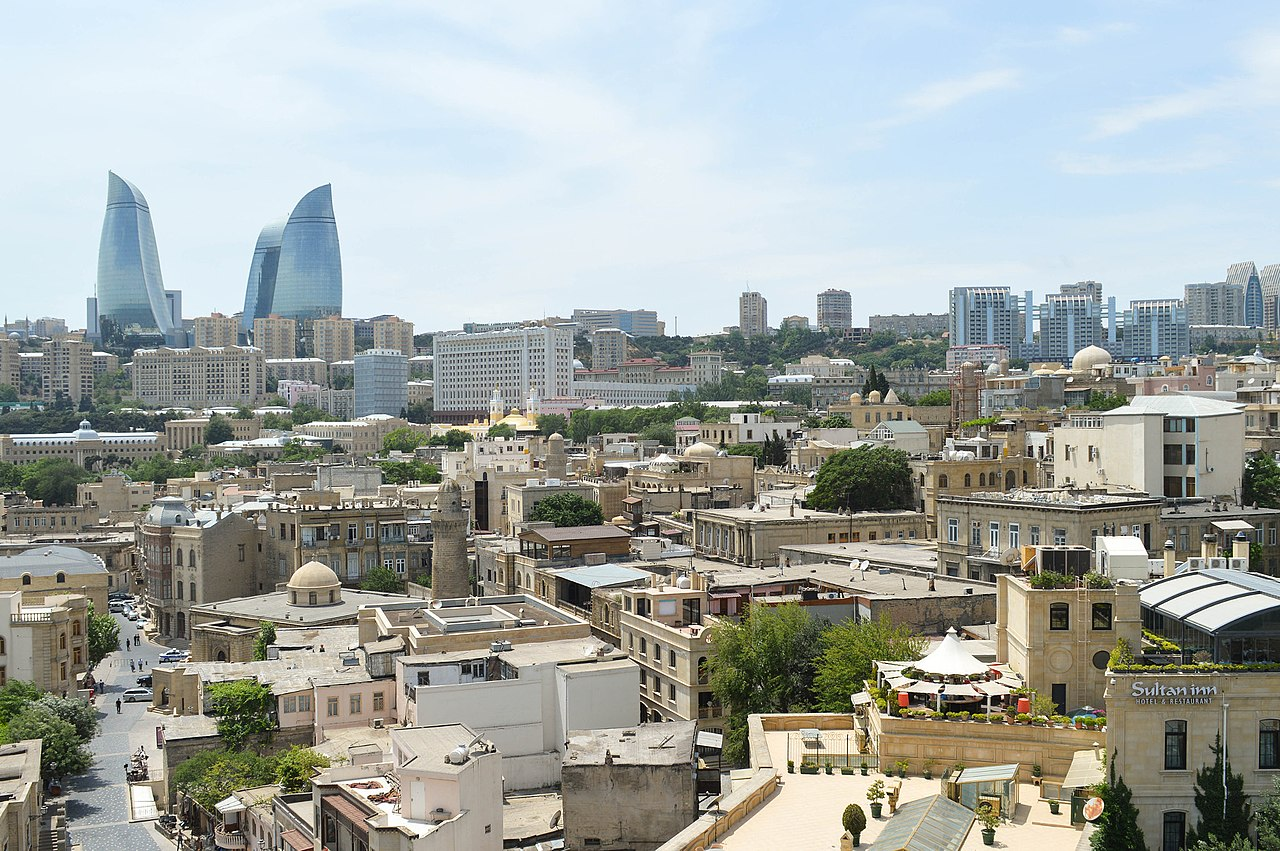
\includegraphics[width=12cm, height=8cm]{img/baku02.jpeg}
\end{frame}

\begin{frame}{Baku}
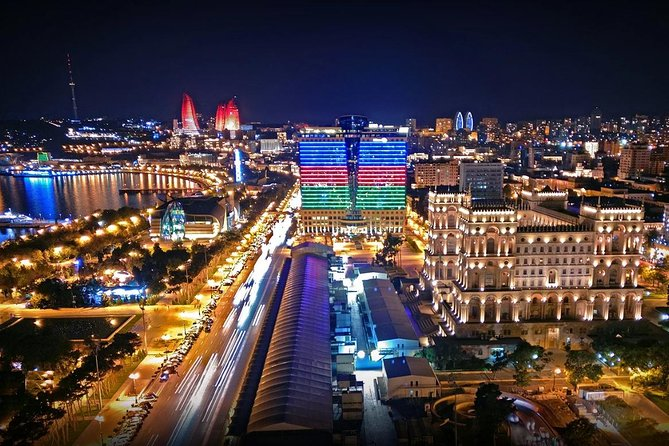
\includegraphics[width=12cm, height=8cm]{img/baku03.jpg}
\end{frame}

\begin{frame}{Cities}
\begin{alertblock}{Ganja}
\justifying Ganja is the second largest city of Azerbaijan, located on the banks of Ganja river on the northern slopes of Less Caucasus range about 375 km west from Baku. Ganja is one of the oldest cities in the Caucasus, and has long been one of the most important in Azerbaijan. Ganja population - 332,600.
\end{alertblock}
\end{frame}

\begin{frame}{Ganja}
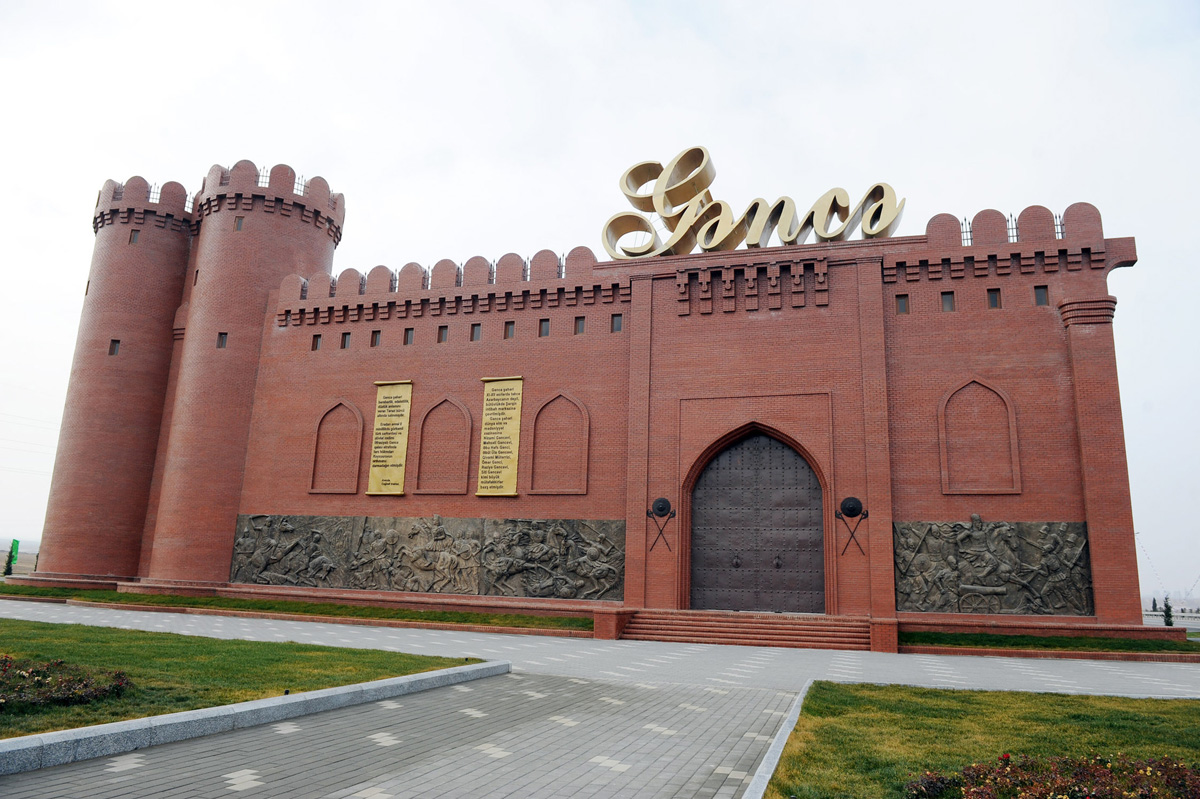
\includegraphics[width=12cm, height=8cm]{img/gence01.jpg}
\end{frame}

\begin{frame}{Ganja}
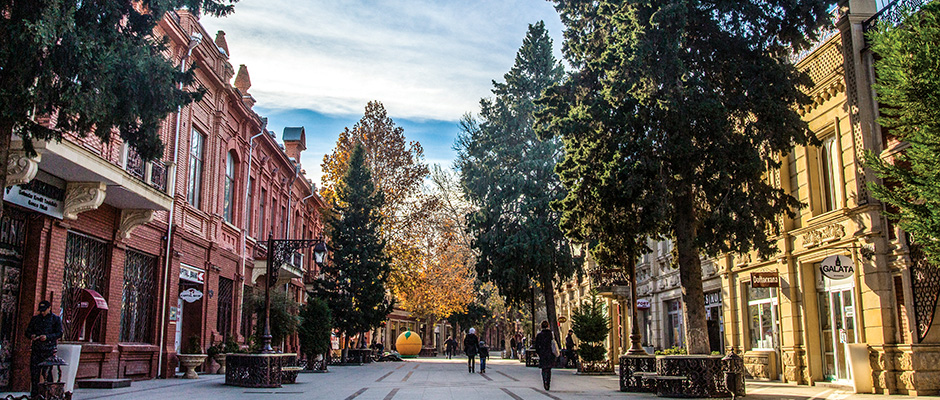
\includegraphics[width=12cm, height=8cm]{img/gence02.jpg}
\end{frame}

\begin{frame}{Ganja}
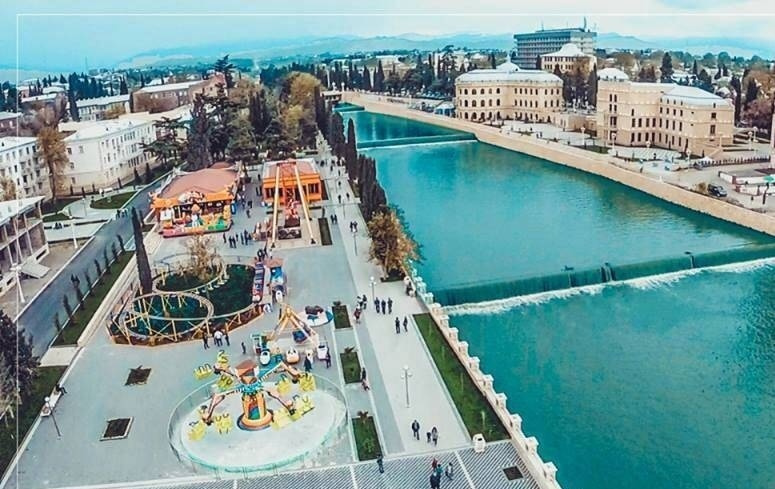
\includegraphics[width=12cm, height=8cm]{img/gence03.jpg}
\end{frame}

\begin{frame}{Cities}
\begin{alertblock}{Sumqayit}
\justifying The third biggest city in Azerbaijan after Baku and Ganja. Sumqayit is located close to the Caspian Sea, 31 km away from the capital city of Baku.
Sumqayit supports a number of heavy industries including metallurgical and chemical plants. Sumqayit population - 341,200.
\end{alertblock}
\end{frame}

\begin{frame}{Sumqayit}
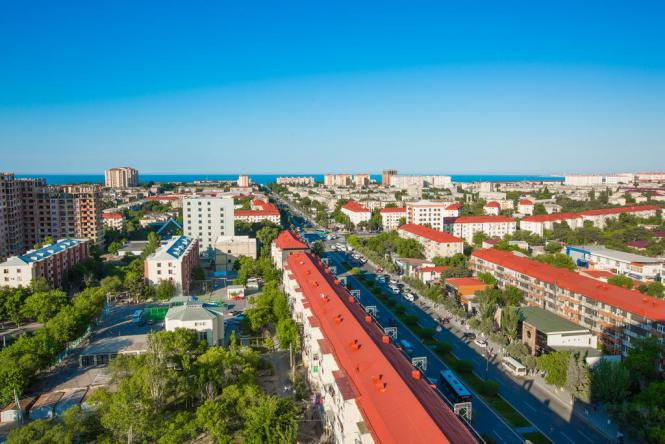
\includegraphics[width=12cm, height=8cm]{img/sum01.jpg}
\end{frame}

\begin{frame}{Sumqayit}
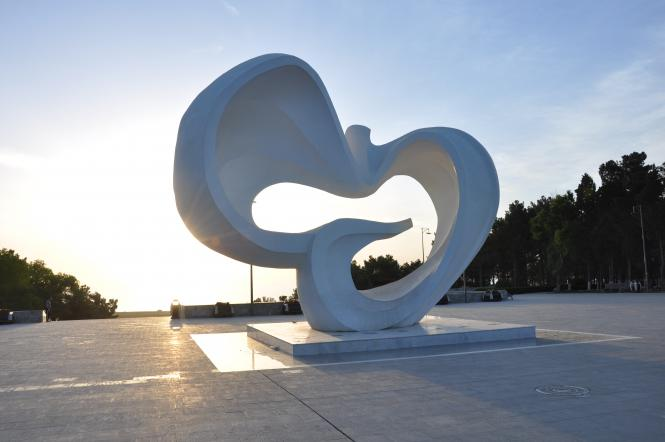
\includegraphics[width=12cm, height=8cm]{img/sum02.jpg}
\end{frame}

\begin{frame}{Sumqayit}
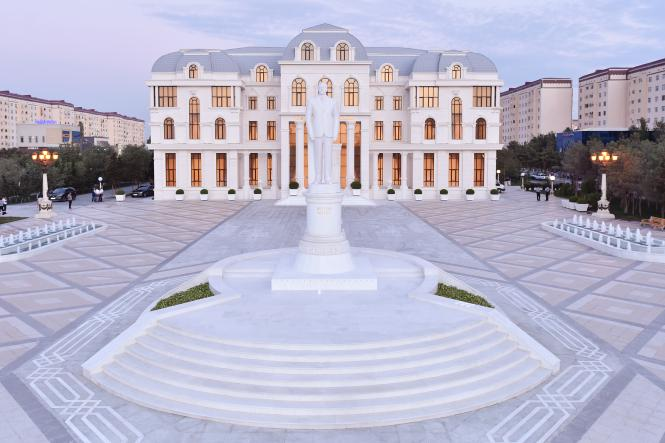
\includegraphics[width=12cm, height=8cm]{img/sum03.jpg}
\end{frame}

\begin{frame}{Landscape}
\begin{alertblock}{Landscape}
Azerbaijan is home to a vast variety of landscapes.
Over half of Azerbaijan's landmass consists of mountain ridges, crests, yailas, and plateaus.
9 out of 11 existing climate zones are present in
Azerbaijan.
\end{alertblock}
\end{frame}


\begin{frame}{Landscape}
\centering
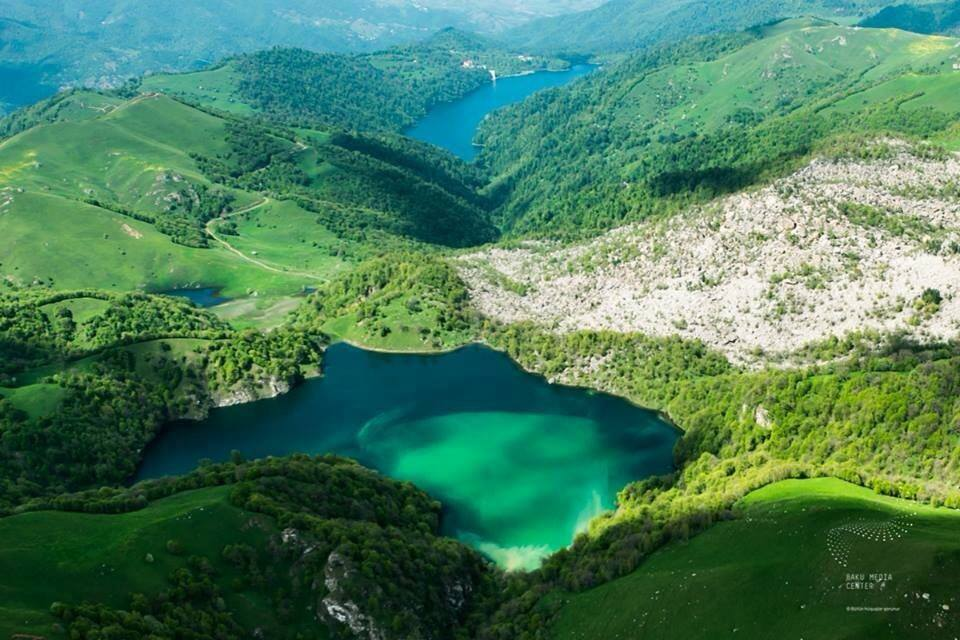
\includegraphics[width=5cm, height=3.9cm]{img/lake01.jpg}
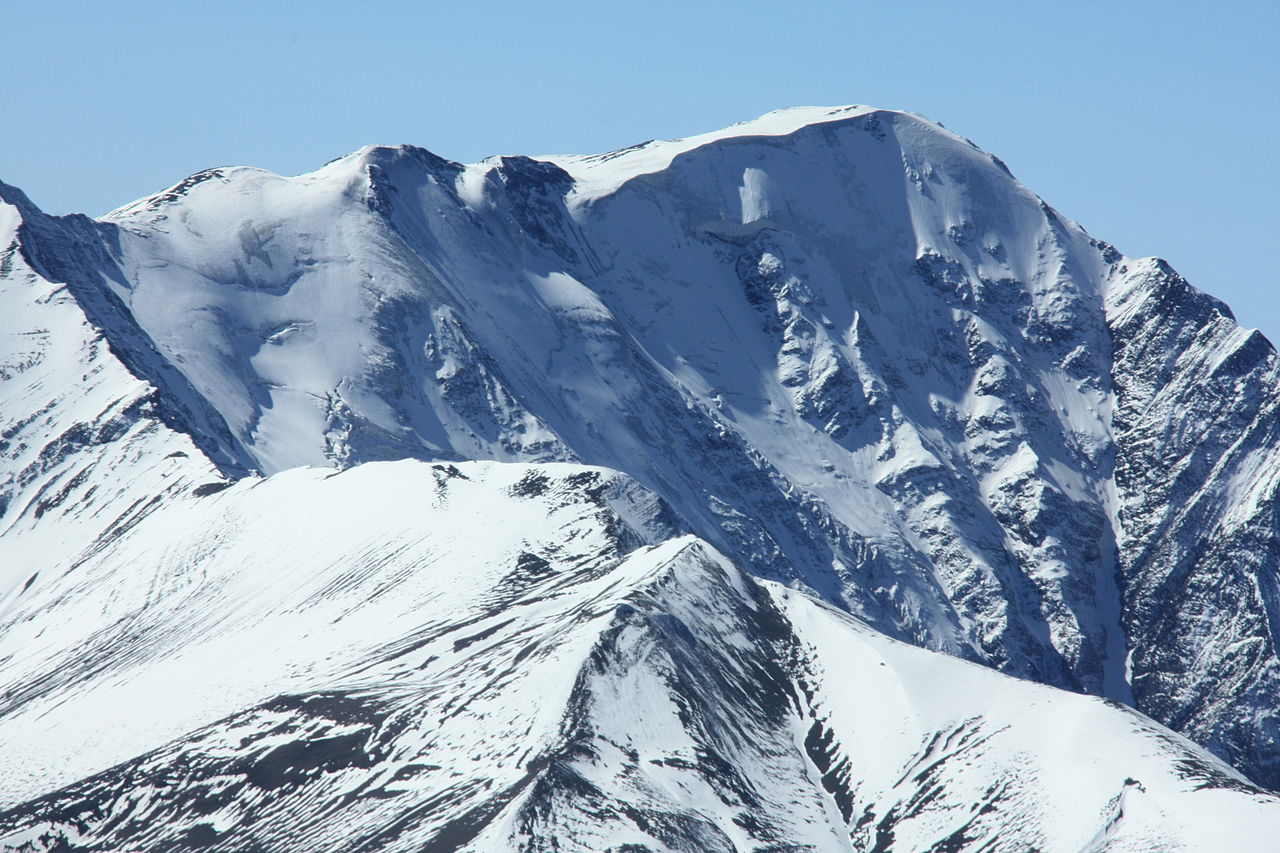
\includegraphics[width=5cm, height=3.9cm]{img/mount01.jpg}

\vspace{0.5mm}
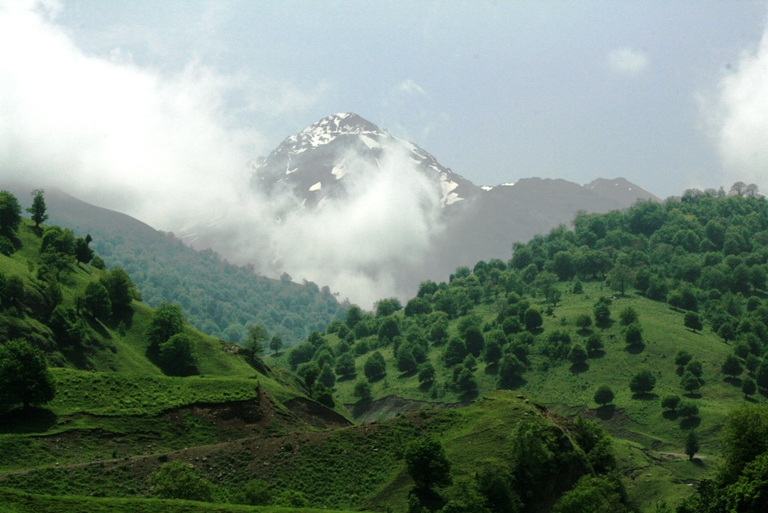
\includegraphics[width=5cm, height=3.9cm]{img/mount02.jpg}
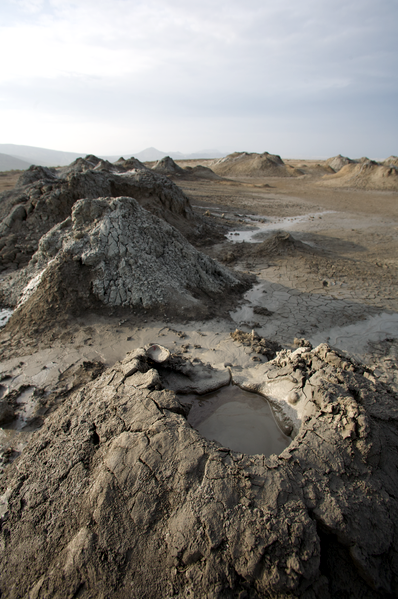
\includegraphics[width=5cm, height=3.9cm]{img/vul01.png}
\end{frame}

\begin{frame}{Cuisine}
\begin{alertblock}{Cuisine}
\justifying Azeri food features a spread of different dishes such as plov (saffron-covered rice, which also happens to be the national dish), a variety of kebabs and shashlik, an array of seafood dishes, fresh-fruits and vegetables, sumptuous soups, and lots of other dishes cooked using fresh, aromatic herbs and spices.
\end{alertblock}
\end{frame}

\begin{frame}{Cuisine}
\centering
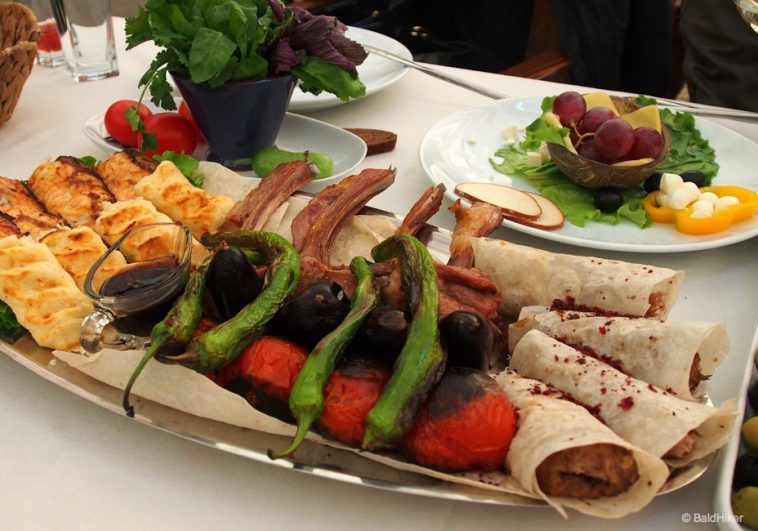
\includegraphics[width=5cm, height=3.9cm]{img/cus01.jpg}
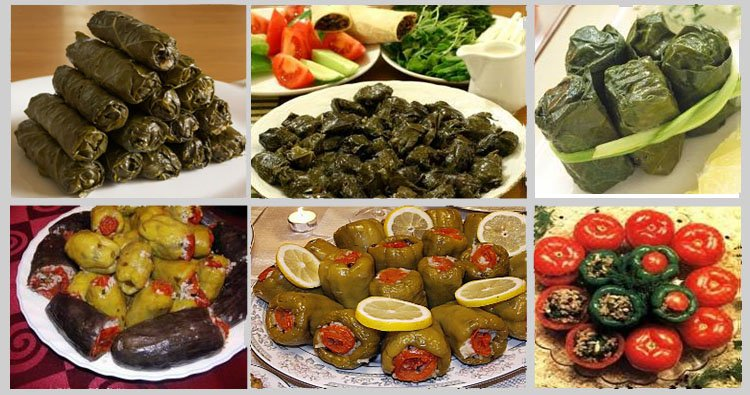
\includegraphics[width=5cm, height=3.9cm]{img/cus02.jpg}

\vspace{0.5mm}
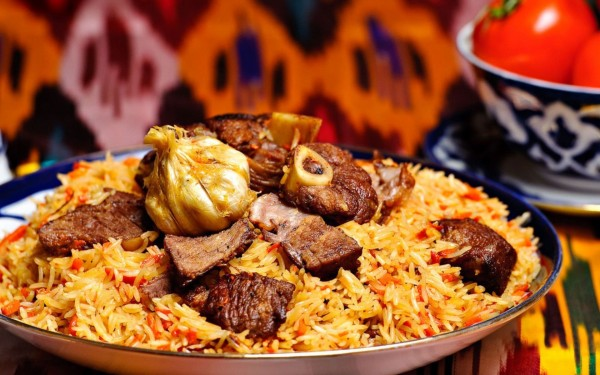
\includegraphics[width=5cm, height=3.9cm]{img/cus03.jpg}
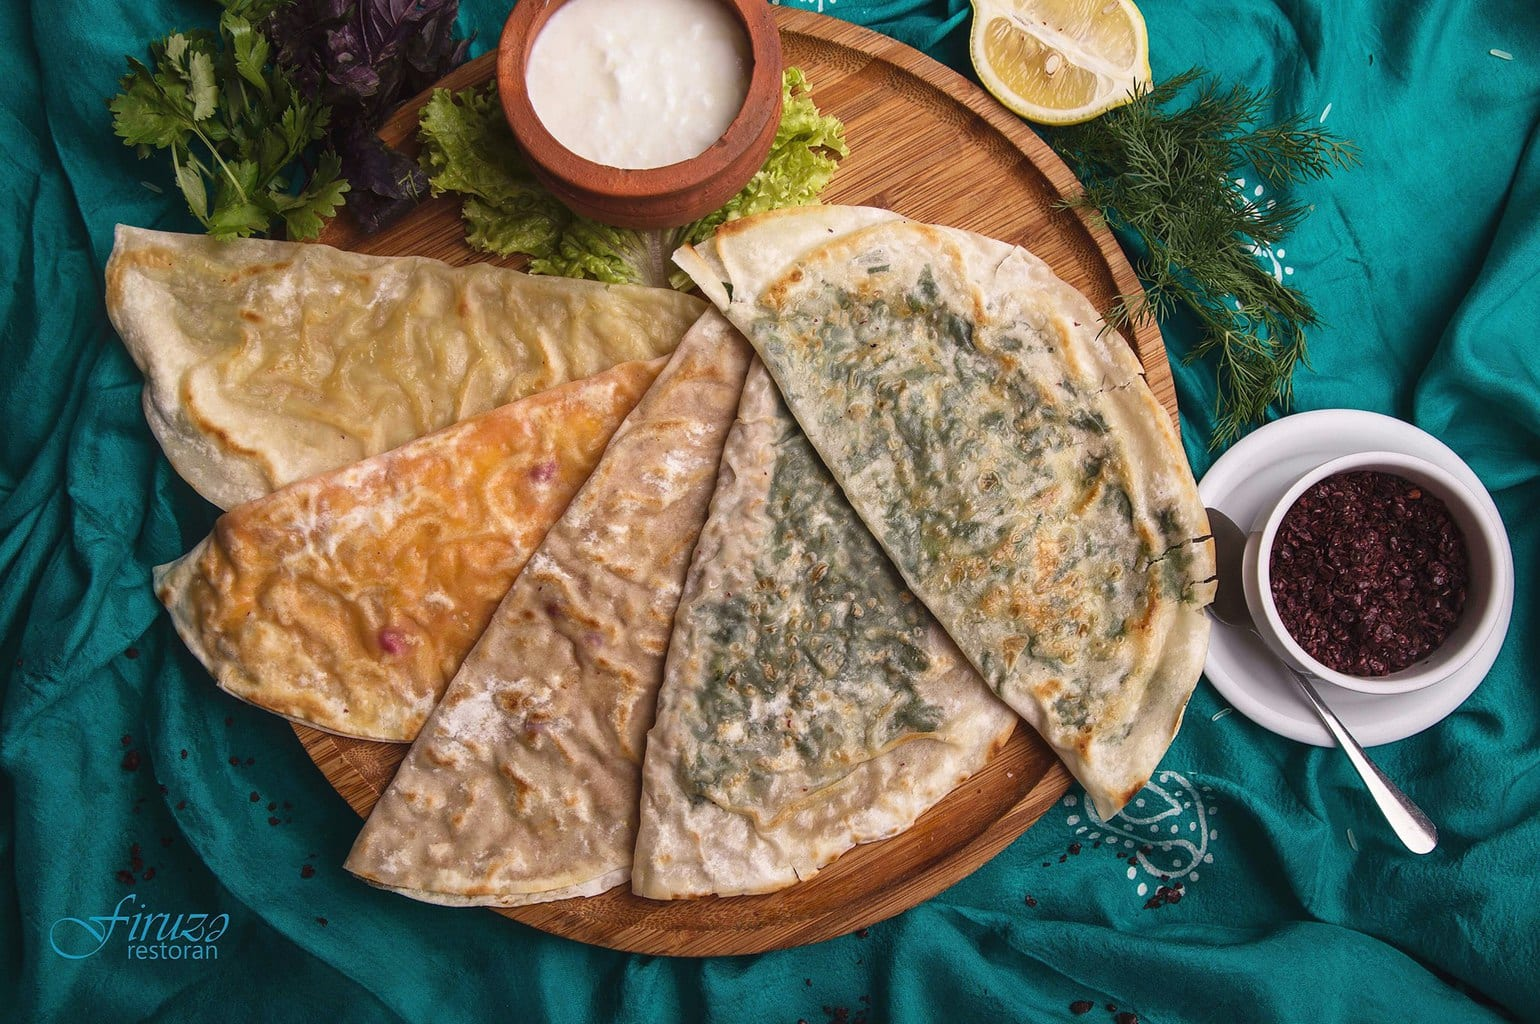
\includegraphics[width=5cm, height=3.9cm]{img/cus04.jpg}
\end{frame}


\end{document}
